%!TEX root = base.tex

\chapter{Background}

This report touches a wide range of topics, technologies and systems, and this
chapter briefly introduces them and provides a summary of their, for this
report, key points.

\section{IEEE 802.11}

The now ubiquitous family of wireless network protocols and ammendments, such
as IEEE 802.11g and IEEE 802.11x, commonly known as Wi-Fi. More specifically
IEEE 802.11 defines the PHY and MAC layers of the network stack. Each
ammendment introduces additions, redactions and changes to these layers. It's
best to read the following overview with this in mind. For a more complete
definition of the \emph{distributed coordination function} (DCF) the reader is
referred to \cite{654749}, \cite{5307322} and \cite{6687187}. 

IEEE 802.11 implements a \emph{Carrier-Sense Multiple Access} (CSMA) medium
access control (MAC) scheme with a binary exponential backoff algorithm for
\emph{collision avoidance} (CA). The algorithm is run locally on each network
node and is called the \emph{Distributed Coordination Function} (DCF). 

When nodes in a IEEE 802.11 network wants to transmit data they must first
listen on the channel and wait until no activity has been detected for a
duration, the \emph{DCF Interframe Space} (DIFS). Since this effectively
synchronizes the nodes waiting to transmit, a random delay is introduced to
desynchronise nodes. This delay is called back-off time
($T_{\mathit{backoff}}$) and belongs to the \emph{collision avoidance}
algorithm which requires time to be quantized into discrete \emph{time-slots},
each $9$ to $50$ $\mu s$ long, depending on the standard. 

While in back-off, nodes listen on the medium for a full \emph{slot} and, if
no activity has been sensed, decrements the back-off counter. If nodes detect
activity on the medium during a slot, the counter is not decremented (counter
freezing). Upon reaching zero the node may attempt to (re)transmit. If no
\texttt{ACK} has been received after a certain duration (\texttt{ACK-Timeout})
the node waits another DIFS, enters further back-off (see \ref{fig:cwsizes})
and restarts its journey back to zero again. The node has a fixed number of
attempts to retransmit the frame, \texttt{ShortRetryLimit} \cite{654749}, and
drops the frame once exceeded.

\begin{figure}
\center
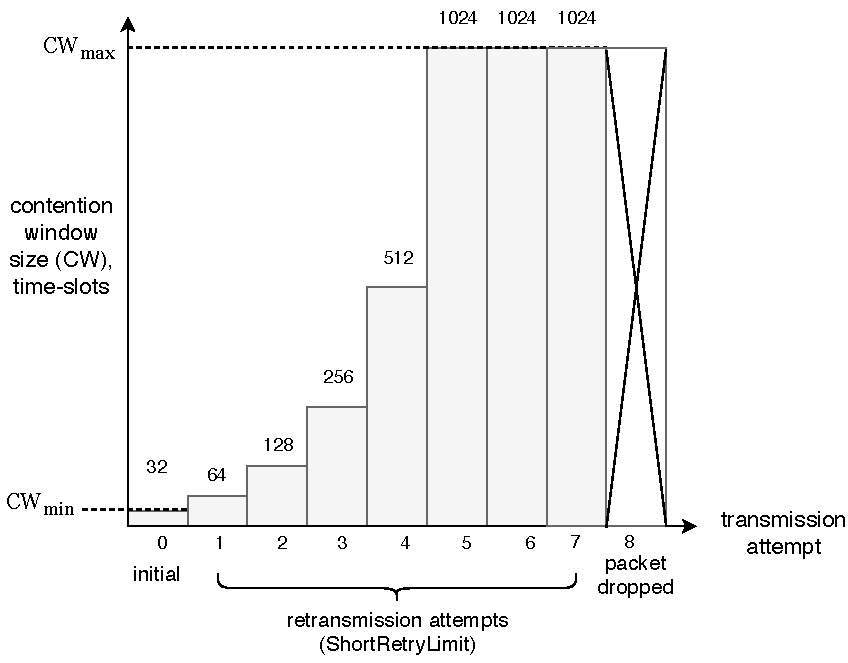
\includegraphics[width=0.8\textwidth]{images/contention-window-sizes.pdf}
\caption{Contention window size increases exponentially on each retransmission attempt, from $\mathit{CW}_{min}$ up to $\mathit{CW}_{max}$}
\label{fig:cwsizes}
\end{figure}

Time spent in back-off for each (re)transmission attempt $j$ is described in
equation \ref{eq:tbackoff}, where \emph{SlotTime} is defined in \cite{654749}
and $\mathcal{U}(0,W_j-1)$ is a uniformly sampled value between $0$ and the
contention window size $W_{j}-1$, i.e. the maximum number of time-slots
(exclusive, since 0 is a valid back-off counter). 

The contention window \emph{size} at transmission attempt $j$, $W_{j}$, is
defined in equation \ref{eq:cwj}, where $L$ is the number of retransmssion
attempts before a packet is dropped (\texttt{ShortRetryLimit}),
$\mathit{CW}_{min}$ and $\mathit{CW}_{max}$ are minimum and maximum number of
time-slots of the \emph{contention window}, respectively, and $m$ is $\log_2
\frac{\mathit{CW}_{max}}{\mathit{CW}_{min}}$. The defined values of $j$ are
the initial attempt ($j=0$) and an extra $L$ attempts before termination,
which resolves to $0 \leq j \leq L$.

\begin{equation} \label{eq:tbackoff}
T^j_{\mathit{backoff}} = \mathit{SlotTime} \times \mathcal{U}(0,W_j-1)
\end{equation}

\begin{equation} \label{eq:cwj}
W_j = \left\{
	\begin{array}{ll}
		2^j \mathit{CW}_{min}  & \mbox{if } 0 \leq j < m, \\
		\mathit{CW}_{max}      & \mbox{if } m \leq j \leq L
	\end{array}
\right.
\end{equation}

The description above details one of three multiple access schemes in IEEE
802.11—``basic mode''. During CSMA/CA each node listens for activity locally
and can therefore fail to detect nodes whose signal is too weak to be
received, causing what's known as the \emph{hidden node} problem. In IEEE
802.11, only the access point (AP) is guaranteed to have knowledge of all
connected stations (STAs). 

The second multiple access scheme requires that STAs first acquire the right
to transmit, using a \emph{request-to-send} (RTS) message. If the STA is given
permission, the AP will respond with a \emph{clear-to-send} (CTS) message.
This access scheme is called RTS/CTS and increases performance in scenarios
with multiple ``hidden nodes''. The RTS/CTS protocol assumes that all STAs 
have similar tx/rx capabilities.

An overview of the required interframe spaces (IFS) and protocol packets for 
``basic'' and ``RTS/CTS'' modes can be found in Figure \ref{fig:timings}. 

\begin{figure}
\center
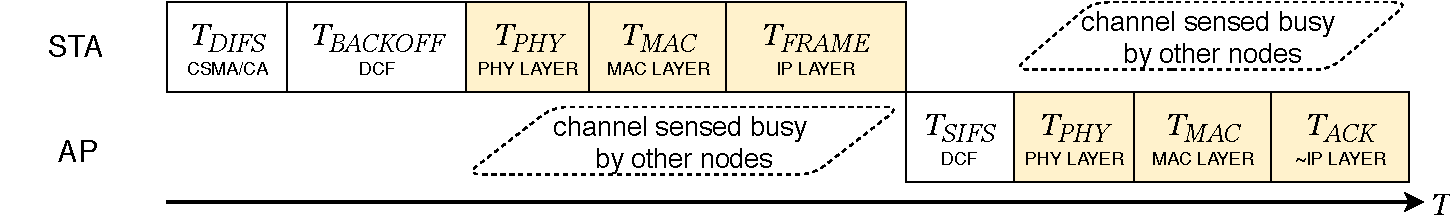
\includegraphics[width=0.8\textwidth]{images/time-overview.pdf}
\caption{Time overview of a successful frame transmission and response in ``basic mode'' and ``RTS/CTS mode''}
\label{fig:timings}
\end{figure}


\section{Linux Networking}

The Linux kernel has a complex networking subsystem which is beyond the scope
of this report to detail. A schematic, high level view of a packet's way from 
userspace program, through the kernel and into the network interface responsible 
for physically transmitting it, can be found in Figure \ref{fig:linux_egress}. 
There are 5 main components in the figure: userspace, kernel, sockets, queueing 
discipline (qdisc), driver and network interface card (NIC). Each component is
more complex than described and interested readers are referred to \cite{knet},
\cite{pcsending} and \cite[Chapter~17]{ldd}.

\begin{enumerate}
	
	\item A \textbf{userspace} program initializes, binds and attempts to send
	data through a socket using system calls \texttt{socket(2)}, \texttt{bind(2)} 
	and \texttt{send(2)}, \texttt{sendto(2)} or \texttt{sendmsg(2)}.

	\item The \textbf{linux kernel} allocates a per-socket kernel buffer (\texttt{skb}), 
	where related kernel (bookeeping), socket and packet data is stored. The initial
	size of the \texttt{skb} depends on the \texttt{net.core.wmem\_default} and 
	\texttt{net.core.wmem\_max} kernel parameters. The \texttt{send(2)}, \texttt{sendto(2)} and 
	\texttt{sendmsg(2)} syscalls must requests memory from the \texttt{skb} belonging to the 
	socket in use, before proceeding through the packet processing stack (UDP/TCP, IP, etc) 
	and finally enqueuing the packet in the queueing discipline (qdisc). The syscalls
	either blocks or fails, with \texttt{EWOULDBLOCK} or \texttt{EAGAIN}, when the 
	packet does not fit into the send buffer (\texttt{skb}), depending on the I/O 
	mode of the socket (blocking or non-blocking).

	\item The \textbf{queueing discipline} (qdisc) system is the internal queueing system 
	of the linux kernel. A qdisc is a configurable, per-network device queueing system with a 
	default ``pfifo\_fast'', prioritized fifo, queue, see Figure \ref{fig:pfifofast}. As 
	packets arrive the qdisc signals the driver, using a scheduler, that data is available. 
	The qdisc can be queried and configured using the \texttt{tc(8)} (traffic control),
	\texttt{ip(8)} and \texttt{ifconfig(8)} programs. 

	\item The \textbf{driver} interfaces between the kernel and network device hardware and
	can be considered a program itself (kernel module). Drivers considered in this thesis
	all use an internal ring buffer for egress packets, called the ``TX-Ring''. The driver
	pulls packets from the qdisc into the ``TX-Ring'' and signals the NIC that packets are
	ready to be sent. Memory consumed by a packet is defered until some time after transmit
	or drop. The Linux kernel supports a feature called ``packet taps'' which enable kernel
	modules to capture packets as they enter or exit the kernel. The outbound taps are called 
	at the end of the Linux kernel's outbound packet processing path, right before control of 
	the packet is handed over to the driver.

	\item The \textbf{network interface card} (NIC) which primarily sends and receives packets. 
	The internal design documents of many NICs are not publicly available and open source
	drivers only hint at the design of important subsystems, such as buffers and prefetchers. 

\end{enumerate}

\begin{figure}
\center
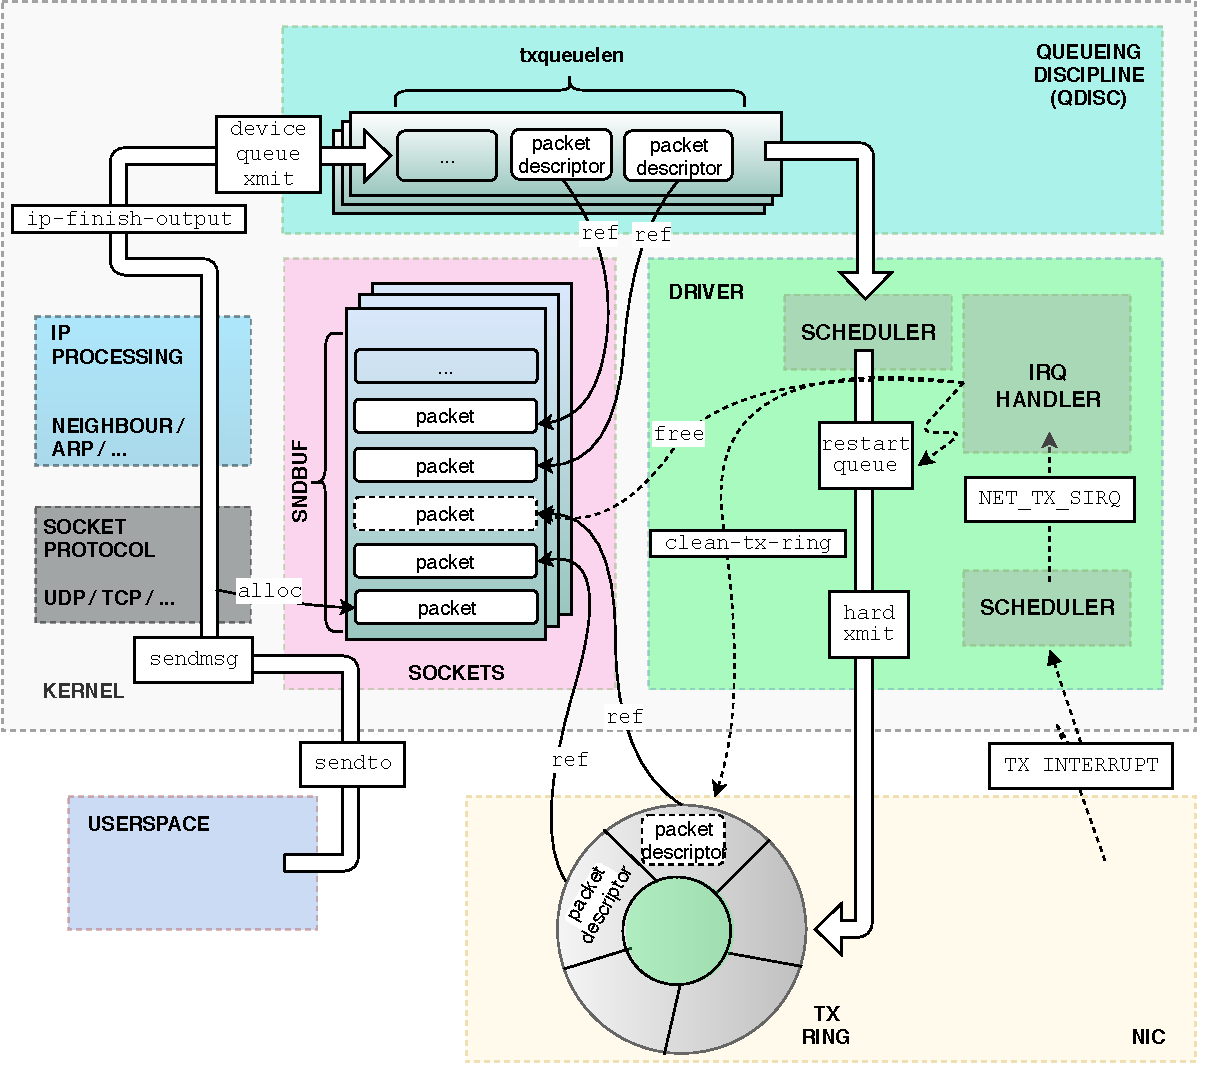
\includegraphics[width=0.9\textwidth]{images/linux-egress-overview.pdf}
\caption{TG799 router and measurement antenna side by side, 1 meter from laptop}
\label{fig:linux_egress}
\end{figure}

\begin{figure}
\center
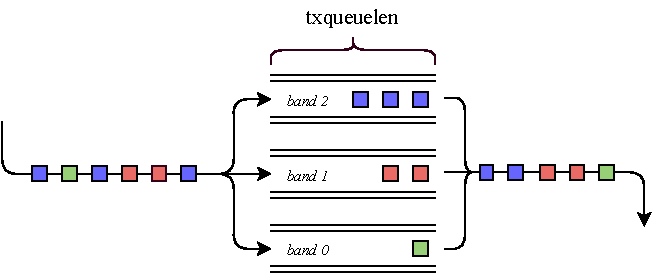
\includegraphics[width=0.8\textwidth]{images/pfifo-fast-queue.pdf}
\caption{An overview of the default queueing discipline, \texttt{pfifo\_fast}. Packets are enqueued into band 0, 1 or 2 depending on queue configuration and packet TOS bits. Band 0 is highest priority and band 2 lowest. Queue length is counted in number of packets.}
\label{fig:pfifofast}
\end{figure}

\section{TG799-vac}

The OpenWrt-based router examined in this thesis, see Figure \ref{fig:tg799}, is
commonly known as TG799-vac. It is manufactured by Technicolor and uses Broadcom 
and Quantenna modems. It is, as of time of writing, the default router provided 
by many Swedish ISPs, and therefore widely deployed.

A custom firmware was used to gain root access and install the iperf3 module.

\begin{figure}
\center
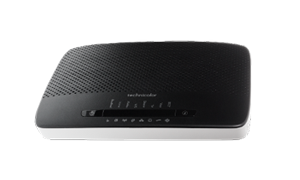
\includegraphics[width=0.5\textwidth]{images/tg799.png}
\caption{The TG799 router from Technicolor}
\label{fig:tg799}
\end{figure}

\section{ubus - the OpenWrt micro bus architecture}

A program which acts as an interface to the bus daemon, \texttt{ubusd}.
Proprietary modules are registered by namespaces in \texttt{ubusd} and 
\texttt{ubus} enables simple interaction with the registered objects using 
JSON. A usage example can be found in Listing \ref{lst:ubusex}.

This tool was used to read statistics from the TG799-vac device,
such as tx rates, packet counters and medium availability.

\begin{lstlisting}[language=bash,caption={Example ubus usage},label=lst:ubusex]
$ ubus call wireless.accesspoint get
{
        "ap0": {
                "ssid": "wl0",
                "station_history": 1,
                "max_assoc": 0,
                ... (omitted)
	},
	... (omitted)
}
\end{lstlisting}

\section{Wireshark}

Wireshark is a well-known program for capturing and inspecting network data,
and has been used extensively during the research and development of this
thesis. On Linux, it uses \texttt{libpcap} to register a packet tap for live
capture. Due to the way packet taps work in the Linux kernel Wireshark cannot
timestamp the moment the packet physically was transmitted, unless the network
interface card explicitly supports hardware timestamps. None of the NICs used
in this thesis have this feature.

\section{jana}

A program, developed by the author of this thesis, for running network tests.
Specifically, network tests using expontential, uniform and gamma distributed
packet send rate and payload size. This is in contrast to more powerful tools
such as \texttt{pktgen} and \texttt{trafgen}, which offer better performance
and more per-packet control.